\newpage
\newcommand{\rhok}[0]{\rho_\text{K}}
\subsection{Kugelfallviskosimeter}
	\subsubsection{Viskosität}
		Die Position-Zeit Daten sind im \gnuplot{} geplottet (Siehe Appendix \ref{appdx:tvtwo}) und eine Kurveanpassung zur $y = mt + c$ durchgeführt. Da alle Positionen manuell bestimmt sind, ist einen Fehler von $\Delta y = \pm \SI{5}{\milli\meter}$ dazu addiert. Es ist davon ausgegangen, dass die Kugeln mit konstanten Geschwindigkeit durch das Spülmittel fällt, was möglicherweise wegen der Blase hinter der Kugel nicht der Fall ist:
		\begin{figure}[H]
			\centering
			\captionsetup{width=0.8\linewidth, justification=centering}
			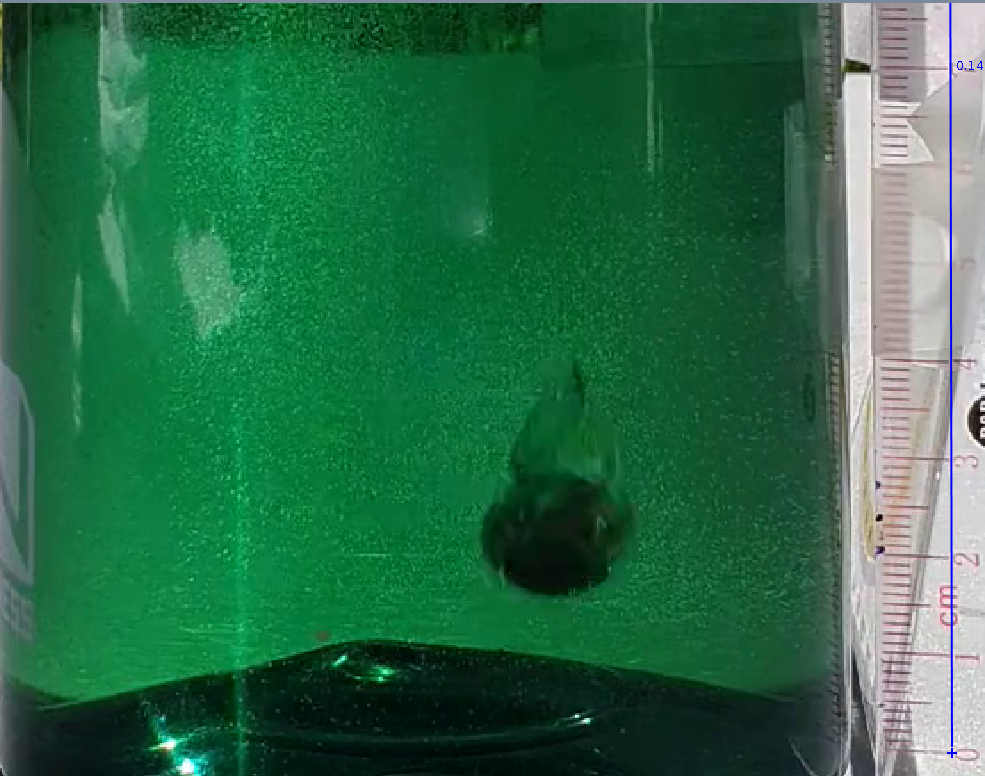
\includegraphics[width=0.5\linewidth]{tv2-bubble.png}
			\caption{Blase hinter der Stahkugel}
			\vspace{-1.25em}
			\label{fig:tv2-bubble}
		\end{figure}
		\begin{figure}[H]
			\centering
			\vspace{-1.25em}
			\captionsetup{width=0.8\textwidth, justification=centering}
			\resizebox{\linewidth}{!}{% GNUPLOT: LaTeX picture with Postscript
\begingroup
  \makeatletter
  \providecommand\color[2][]{%
    \GenericError{(gnuplot) \space\space\space\@spaces}{%
      Package color not loaded in conjunction with
      terminal option `colourtext'%
    }{See the gnuplot documentation for explanation.%
    }{Either use 'blacktext' in gnuplot or load the package
      color.sty in LaTeX.}%
    \renewcommand\color[2][]{}%
  }%
  \providecommand\includegraphics[2][]{%
    \GenericError{(gnuplot) \space\space\space\@spaces}{%
      Package graphicx or graphics not loaded%
    }{See the gnuplot documentation for explanation.%
    }{The gnuplot epslatex terminal needs graphicx.sty or graphics.sty.}%
    \renewcommand\includegraphics[2][]{}%
  }%
  \providecommand\rotatebox[2]{#2}%
  \@ifundefined{ifGPcolor}{%
    \newif\ifGPcolor
    \GPcolortrue
  }{}%
  \@ifundefined{ifGPblacktext}{%
    \newif\ifGPblacktext
    \GPblacktexttrue
  }{}%
  % define a \g@addto@macro without @ in the name:
  \let\gplgaddtomacro\g@addto@macro
  % define empty templates for all commands taking text:
  \gdef\gplbacktext{}%
  \gdef\gplfronttext{}%
  \makeatother
  \ifGPblacktext
    % no textcolor at all
    \def\colorrgb#1{}%
    \def\colorgray#1{}%
  \else
    % gray or color?
    \ifGPcolor
      \def\colorrgb#1{\color[rgb]{#1}}%
      \def\colorgray#1{\color[gray]{#1}}%
      \expandafter\def\csname LTw\endcsname{\color{white}}%
      \expandafter\def\csname LTb\endcsname{\color{black}}%
      \expandafter\def\csname LTa\endcsname{\color{black}}%
      \expandafter\def\csname LT0\endcsname{\color[rgb]{1,0,0}}%
      \expandafter\def\csname LT1\endcsname{\color[rgb]{0,1,0}}%
      \expandafter\def\csname LT2\endcsname{\color[rgb]{0,0,1}}%
      \expandafter\def\csname LT3\endcsname{\color[rgb]{1,0,1}}%
      \expandafter\def\csname LT4\endcsname{\color[rgb]{0,1,1}}%
      \expandafter\def\csname LT5\endcsname{\color[rgb]{1,1,0}}%
      \expandafter\def\csname LT6\endcsname{\color[rgb]{0,0,0}}%
      \expandafter\def\csname LT7\endcsname{\color[rgb]{1,0.3,0}}%
      \expandafter\def\csname LT8\endcsname{\color[rgb]{0.5,0.5,0.5}}%
    \else
      % gray
      \def\colorrgb#1{\color{black}}%
      \def\colorgray#1{\color[gray]{#1}}%
      \expandafter\def\csname LTw\endcsname{\color{white}}%
      \expandafter\def\csname LTb\endcsname{\color{black}}%
      \expandafter\def\csname LTa\endcsname{\color{black}}%
      \expandafter\def\csname LT0\endcsname{\color{black}}%
      \expandafter\def\csname LT1\endcsname{\color{black}}%
      \expandafter\def\csname LT2\endcsname{\color{black}}%
      \expandafter\def\csname LT3\endcsname{\color{black}}%
      \expandafter\def\csname LT4\endcsname{\color{black}}%
      \expandafter\def\csname LT5\endcsname{\color{black}}%
      \expandafter\def\csname LT6\endcsname{\color{black}}%
      \expandafter\def\csname LT7\endcsname{\color{black}}%
      \expandafter\def\csname LT8\endcsname{\color{black}}%
    \fi
  \fi
    \setlength{\unitlength}{0.0500bp}%
    \ifx\gptboxheight\undefined%
      \newlength{\gptboxheight}%
      \newlength{\gptboxwidth}%
      \newsavebox{\gptboxtext}%
    \fi%
    \setlength{\fboxrule}{0.5pt}%
    \setlength{\fboxsep}{1pt}%
\begin{picture}(8640.00,5760.00)%
    \gplgaddtomacro\gplbacktext{%
      \csname LTb\endcsname%%
      \put(814,704){\makebox(0,0)[r]{\strut{}$-70$}}%
      \put(814,1332){\makebox(0,0)[r]{\strut{}$-60$}}%
      \put(814,1960){\makebox(0,0)[r]{\strut{}$-50$}}%
      \put(814,2588){\makebox(0,0)[r]{\strut{}$-40$}}%
      \put(814,3215){\makebox(0,0)[r]{\strut{}$-30$}}%
      \put(814,3843){\makebox(0,0)[r]{\strut{}$-20$}}%
      \put(814,4471){\makebox(0,0)[r]{\strut{}$-10$}}%
      \put(814,5099){\makebox(0,0)[r]{\strut{}$0$}}%
      \put(946,484){\makebox(0,0){\strut{}$0,1$}}%
      \put(1714,484){\makebox(0,0){\strut{}$0,2$}}%
      \put(2482,484){\makebox(0,0){\strut{}$0,3$}}%
      \put(3250,484){\makebox(0,0){\strut{}$0,4$}}%
      \put(4018,484){\makebox(0,0){\strut{}$0,5$}}%
      \put(4787,484){\makebox(0,0){\strut{}$0,6$}}%
      \put(5555,484){\makebox(0,0){\strut{}$0,7$}}%
      \put(6323,484){\makebox(0,0){\strut{}$0,8$}}%
      \put(7091,484){\makebox(0,0){\strut{}$0,9$}}%
      \put(7859,484){\makebox(0,0){\strut{}$1$}}%
    }%
    \gplgaddtomacro\gplfronttext{%
      \csname LTb\endcsname%%
      \put(209,2901){\rotatebox{-270}{\makebox(0,0){\strut{}Torsionswinkel $\phi$ ($\si{\degree}$)}}}%
      \put(4594,154){\makebox(0,0){\strut{}$\sin(\alpha/\si{\degree})$}}%
      \csname LTb\endcsname%%
      \put(7256,4893){\makebox(0,0)[r]{\strut{}$-64,51852I + -0,14015$}}%
      \csname LTb\endcsname%%
      \put(7256,4607){\makebox(0,0)[r]{\strut{}Messpunkte}}%
      \csname LTb\endcsname%%
      \put(4594,5429){\makebox(0,0){\strut{}Torsionswinkel $\phi$ gegen $\sin(\alpha/\si{\degree})$}}%
    }%
    \gplbacktext
    \put(0,0){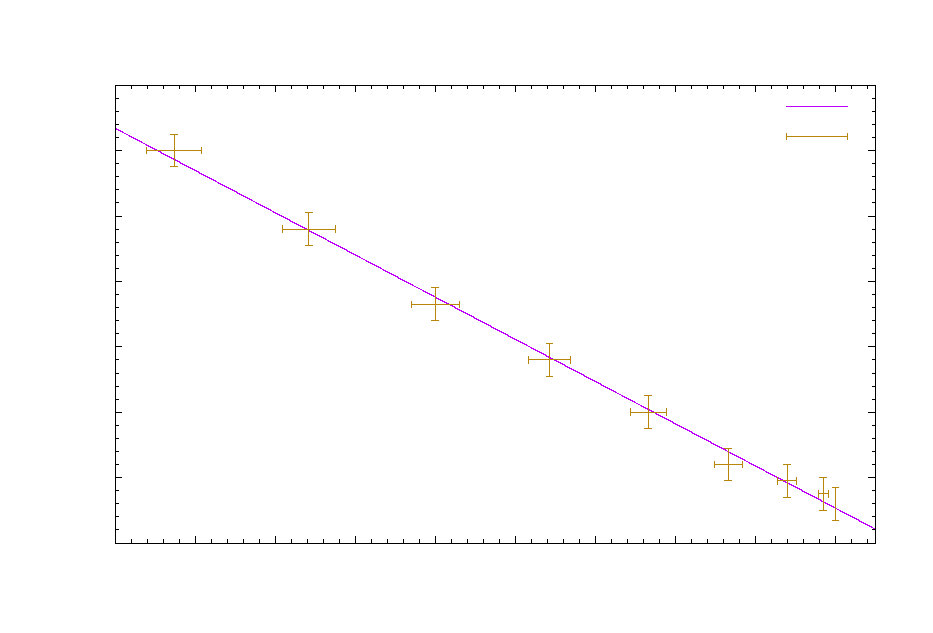
\includegraphics[width={432.00bp},height={288.00bp}]{tv2-plot}}%
    \gplfronttext
  \end{picture}%
\endgroup
}
			\caption{Fall der Stahlkugel im Spülmittel \textattachfile[author={Yudong Sun},color={0 0.404 0.584},description={.zip Datei mit der Messwerten},mimetype={application/zip},timezone={+02'00'}]{./attachments/kugelfallviskosimeter.zip}{\textit{(Daten)}}}
			\vspace{-1em}
		\end{figure}
		Da es zu viele Datenpunkten gibt, sind sie hier ausgelasen. 

		Als Ergebnis erhalten wir:
		\begin{center}
			\begin{tabular}{lrrr}
				\toprule
				Kugel Nr. & $m/\si{\milli\meter\per\second}$ & $c/\si{\milli\meter}$ & $\chi^2_\text{red}$ \\
				\midrule
					$1$ & \num{-1039,02016(711891)} & \num{0,97689(49634)} & \num{0,02365} \\
					$2$ & \num{-1097,64782(458963)} & \num{0,28449(32000)} & \num{0,00983} \\
					$3$ & \num{-1155,39617(568788)} & \num{-0,01640(39657)} & \num{0,01510} \\
					$4$ & \num{-1082,00957(708212)} & \num{0,86551(56196)} & \num{0,03344} \\
					$5$ & \num{-1140,03598(628836)} & \num{0,72630(37788)} & \num{0,01230} \\
					$6$ & \num{-1139,65074(602326)} & \num{0,44495(36195)} & \num{0,01129} \\
					$7$ & \num{-1116,62708(606814)} & \num{0,82640(36465)} & \num{0,01146} \\
					$8$ & \num{-1125,03549(815266)} & \num{0,75324(56842)} & \num{0,03102} \\
					$9$ & \num{-1091,94893(857618)} & \num{1,08144(51536)} & \num{0,02288} \\
				\bottomrule
			\end{tabular}
		\end{center}
		Aus der kleiner $\chi^2_\text{red}$-en sind die Anpassungen gut. $m$ entspricht in diesem Fall die Geschwindigkeit der Kugeln und $c$ die Anfangsgeschwindigkeit bei $t=0$. $c$ soll kleiner als $0$ sein, was hier im Allgemein nicht der Fall ist. Das könnte man wahrscheinlich zur Unsicherheit bei der Punktebestimmung zurückführen.

		Nach geeigneter Rundung erhalten wir den Betrag der Fallgeschwindigkeiten:
		\begin{center}
			\begin{tabular}{lr}
				\toprule
				Kugel Nr. & $v_i/\si{\milli\meter\per\second}$ \\
				\midrule
					\num{1} & \num{1039(8)} \\
					\num{2} & \num{1098(5)} \\
					\num{3} & \num{1155(6)} \\
					\num{4} & \num{1082(8)} \\
					\num{5} & \num{1140(7)} \\
					\num{6} & \num{1140(7)} \\
					\num{7} & \num{1117(7)} \\
					\num{8} & \num{1125(9)} \\
					\num{9} & \num{1092(9)} \\
				\bottomrule
			\end{tabular}
		\end{center}
		Wir berechnen nun den Mittelwert, die Unsicherheit des Mittelwerts und die Standardabweichung der Fallgeschwindigkeit. Dazu sind die Funktionen \texttt{AVERAGE} und \texttt{STDEV.S} verwendet. Die Unsicherheit des Mitterwerts ist gegeben durch:
		\begin{equation}
			\Delta \overline{v} = \frac{1}{9} \sqrt{\sum^{9}_{i=1}(\Delta v_i)^2}
		\end{equation}
		Somit haben wir:
		\begin{center}
			\begin{tabular}{lrr}
				\toprule
				Mittelwert & $\overline{v}$ & \SI{1109.8}{\milli\meter\per\second}\\
				Unsicherheit des Mittelwertes & $\Delta\overline{v}$ & \SI{2.5}{\milli\meter\per\second}\\
				Standardabweichung & $s(v)$ & \SI{37}{\milli\meter\per\second}\\
				\bottomrule
			\end{tabular}
		\end{center}
		wobei $\Delta\overline{v}$ und $s(v)$ beides auf 2 signifikanten Ziffern aufgerundet sind. 

		Da die Standardabweichung größer als die Unsicherheit des Mittelwertes ist, nehmen wir die Standardabweichung als Fehler der Fallgeschwindigkeit an und erhalten $v = \SI{1110(40)}{\milli\meter\per\second}$.

		Wir berechnen zunächst die Dichte der Kugeln $\rho_\text{K}$. Es gilt:
		\begin{align} 
			\rhok &= \frac{m}{V} = \frac{m}{\frac{4}{3}\pi r^3} = \frac{3m}{4\pi r^3} = \frac{6m}{\pi (2r)^3} = \frac{6m}{\pi d^3}  \\
			\Delta \rhok &= \rhok \sqrt{
				\left(\frac{\Delta m}{m}\right)^2 +
				\left(3\cdot \frac{\Delta d}{d}\right)^2
			}
		\end{align}
		Mit der Werten:
		\begin{center}
			\begin{tabular}{lrr}
				\toprule
				Variable & Wert & Bedeutung \\
				\midrule
				$m$ & \SI{8.5(2)}{\gram} & Masse einer Kugel \\
				$d$ & \SI{12.7(1)}{\milli\meter} & Durchmesser einer Kugel \\
				\bottomrule
			\end{tabular}
		\end{center}
		erhalten wir:
		\begin{align}
			\rhok &= \frac{6(\SI{8.5e-3}{\kilo\gram})}{\pi (\SI{12.7e-3}{\meter})^3} = \SI{7925.18}{\kilogram\per\meter\cubed} \sigfig{6} \\
			\Delta \rhok &= \frac{6(\SI{8.5e-3}{\kilo\gram})}{\pi (\SI{12.7e-3}{\meter})^3} \sqrt{
				\left(\frac{\SI{0.2}{\gram}}{\SI{8.5}{\gram}}\right)^2 +
				\left(3\cdot\frac{\SI{0.1}{\milli\meter}}{\SI{12.7}{\milli\meter}}\right)^2
			} = \SI{264.235}{\kilogram\per\meter\cubed} \sigfig{6}\\
			\Rightarrow \rhok &= \SI{7930(270)}{\kilogram\per\meter\cubed} = \SI{7.930(270)}{\gram\per\centi\meter\cubed}
		\end{align}
		Dieser Wert stimmen mit der gegebene Dichte von Stahl $\rho = \SI{7.9}{\gram\per\centi\meter\cubed}$ überein.

		Aus der Anleitung und AMW gilt:
		\begin{align}
			\eta &= \frac{2gr^2}{9v}\left(\rhok - \rho_\spuli\right) 
			= \frac{g(2r)^2}{18v}\left(\rhok - \rho_\spuli\right) 
			= \frac{gd^2}{18v}\left(\rhok - \rho_\spuli\right) \\
			\Delta \eta &= \eta \sqrt{
				\left(2\cdot\frac{\Delta d}{d}\right)^2 +
				\left(\frac{\Delta v}{v}\right)^2 +
				\left(\frac{\Delta (\rho_k - \rho_\spuli)}{\rho_k - \rho_\spuli}\right)^2
			} \notag \\
			&= \eta \sqrt{
				\left(2\cdot\frac{\Delta d}{d}\right)^2 +
				\left(\frac{\Delta v}{v}\right)^2 +
				\frac{(\Delta \rho_k)^2 + (\Delta \rho_\spuli)^2}{\left(\rho_k - \rho_\spuli\right)^{2}}
			}
		\end{align}
		Dazu ist die relative Unsicherheit $\Delta \eta/\eta$ gegeben durch:
		\begin{align}
			\frac{\Delta \eta}{\eta} = \sqrt{
				\left(2\cdot\frac{\Delta d}{d}\right)^2 +
				\left(\frac{\Delta v}{v}\right)^2 +
				\frac{(\Delta \rho_k)^2 + (\Delta \rho_\spuli)^2}{\left(\rho_k - \rho_\spuli\right)^{2}}
			}
		\end{align}
		Wir gehen davon aus, dass die Dichte des Spülmittels Temperaturunabhängig ist.
		\newpage
		Mit der Werten:
		\begin{center}
			\begin{tabular}{lrr}
				\toprule
				Variable & Wert & Bedeutung \\
				\midrule
				$d$ & \SI{0.0127(1)}{\meter} & Durchmesser einer Kugel \\
				$v$ & \SI{1.11(4)}{\meter\per\second} & Mittlere Fallgeschwindigkeit  \\
				$\rhok$ & \SI{7930(270)}{\kilogram\per\meter\cubed} & Dichte der Kugel  \\
				$\rho_\spuli$ & \SI{1080(60)}{\kilo\gram\per\meter\cubed} & Dichte des Spülmittels  \\
				$g$ & \SI{9,81}{\meter\per\second\squared} & Erdbeschleunigung  \\
				\bottomrule
			\end{tabular}
		\end{center}
		erhalten wir:
		\begin{align}
			\eta &= \frac{(\SI{9,81}{\meter\per\second\squared}) (\SI{0.0127}{\meter})^2}{18(\SI{1.11}{\meter\per\second})}
			\left(\SI{7930}{\kilogram\per\meter\cubed}- \SI{1080}{\kilo\gram\per\meter\cubed}\right) \notag \\
			&= \SI{0.542465}{\pascal\second} \sigfig{6} \\
			\Delta\eta &= (\SI{0.542465}{\pascal\second}) \sqrt{
				\left(2\cdot\frac{\SI{0.1}{\milli\meter}}{\SI{12.7}{\milli\meter}}\right)^2 +
				\left(\frac{\SI{0.04}{\meter\per\second}}{\SI{1.11}{\meter\per\second}}\right)^2 +
				\frac{(\SI{270}{\kilogram\per\meter\cubed})^2 + (\SI{60}{\kilo\gram\per\meter\cubed})^2}{\left(\SI{7930}{\kilogram\per\meter\cubed} - \SI{1080}{\kilo\gram\per\meter\cubed}\right)^{2}}
			} \notag \\
			&= \SI{0.0306}{\pascal\second} \sigfig{3}
		\end{align}
		Folglich haben wir eine Viskosität von $\eta = \SI{0.54(3)}{\pascal\second} = \SI{540(30)}{\milli\pascal\second}$ erhalten.

	\subsubsection{Diskussion}
		Zusammengefasst:
		\begin{center}
			\begin{tabular}{lrr}
				\toprule
				Quelle & Temperatur$/\si{\celsius}$ & Viskosität$/\si{\milli\pascal\second}$ \\
				\midrule
				Aufstieg von Luftblasen & \num{29(1)} & \num{256(28)} \\
				Kugelfallviskosimeter & \num{33(1)} & \num{540(30)} \\
				Hersteller & ca. \num{20} & \num{1000} \\
				\bottomrule
			\end{tabular}
		\end{center}
		Also unterscheiden sich die Werten signifikant voneinander. Wie im vorherigen Teilversuch wissen wir ohne Zusatzexperiment nicht, ob der Unterschied zwischen der Herstellerangabe und unseren experimentell bestimmten Werten daran liegt, dass die Temperatur unterschiedlich sind. Aber was unerwartet ist, dass die Viskosität, die aus den Kugelfallviskosimeter bestimmt war, deutlich größer als die, die aus den Aufstieg von Luftblasen bestimmt war. Das kann man nicht mit dem Temperatur erklären, da die Temperatur bei diesem Teilversuch etwa größer als den Vorherigen war, also soll die Viskosität kleiner statt größer sein. 

		Es könnte sein, dass es bei dem vorherigen Teilversuch Randeffekte gibt, die die Reibung reduziert haben, was zu einer niedriger Viskosität führen würde. Außerdem waren die Stahlkugeln im Experiment nicht erst im Spülmittel untertaucht, bevor sie losgelassen wurden. Die Anfangsgeschwindigkeiten waren also nicht gut kontrolliert und gesteuert, was möglicherweise einen großen Einfluss auf die Viskosität hatte. 

		Der improvisierte Kugelfallviskosimeter war vermutlich auch zu klein dafür, dass die Kugel eine konstante Geschwindigkeit erreichen kann. Die Geschwindigkeit war ziemlich schnell und die Messzeiten zu kurz, um es feststellen zu können, ob die Kugel wirklich eine konstante Geschwindkeit hat oder sind diese Messpunkte nur eine lineare Approximation, wenn die Zeit sehr kurz sind.

		Die Luftblasen hinter der Kugel deutet auch darauf hin, dass die Strömung turbulent sein könnten. Wir berechnen zunächst die Renoldzahl:
		\begin{align}
			R_e = \frac{v\cdot d \cdot \rho_\spuli}{\eta} = \frac{\SI{1.11}{\meter\per\second}\cdot \SI{0.0127}{\meter} \cdot \SI{1080}{\kilo\gram\per\meter\cubed} }{\SI{0.54}{\pascal\second}} = \num{28.194} \ll 2000
		\end{align}
		Es ist aber hier davon ausgegangen, dass $\eta$ wirklich richtig ist. Somit können die Strömung laminar sein (aus $R_e$), oder turbulent sein (aus Luftblase).

		Hat man die Zeit, das Experiment zu wiederholen, dann sollte die Temperatur möglichst konstant gehalten (bspw. mittels mittels eines Temperierbads). Dann würden die Ergebnisse vielleicht mehr aussagekräftig.